\chapter{Cybersecurity and Society}
\cite{04_Sociology} - 20hrs module\\
Objectives of this module:
\begin{itemize}
    \item Gain an introduction to sociology, its terminology, relevant theories, and risk sociology applicable to Cybersecurity.
    \item Understand the fundamental concepts of cybercrime and cybersecurity from a sociotechnical perspective.
    \item Explore the social, cultural, and organizational dimensions of cybercrime.
    \item Develop skills in identifying, analyzing, and mitagating cyber threats with a focus on social impacts.
\end{itemize}
It is relevant to learn more about cybersecurity in the societal sphere because "Humans are authors within Society".
\section{Sociology, Really?}
\subsection{What is Sociology?}
Some definitions to sociology.

\begin{displayquote}
    The science of social phenomena subject to natural and invariable laws, with goal of discovering these laws.
\end{displayquote}
\hfill -- Auguste Comte 
\newline

This assertion is overly positivist, as it overlooks potential negative impacts and seems somewhat naive. There are no general laws that describe social phenomena. In the modern view, in fact, no laws exist a priori. Some key parameters in Sociology: historical context and humankind.

\begin{displayquote}
    Sociology is the study of human social life, groups and societies.
\end{displayquote}
\hfill -- Sir Anthony Giddens

A post-positivist claim, states that there are no strong natural laws. This perspective is much more dynamic and mechanistic.

\begin{displayquote}
    Sociology is the scientific study of society, including the intricate patterns of \textbf{social behavior, relationships and human interactions}. It is a systematic examination of social institutions, \textbf{cultural norm} and social change, \textbf{using empirical research and critical analysis}. This discipline aims to understand the underlying mechanisms that govern \underline{social order}, dynamics and transformation, ranging from \textbf{individual interactions at the micro level} to \textbf{social structures at the macro level}. 
    Those in sociology investigate various aspects of human life, including social stratification, movement and change, with an emphasis on \textbf{how collective and individual behavior shapes and is shaped} by the broader social context.
\end{displayquote}
\hfill -- ChatGpt

\subsection{Ethics and Epistemic}

The main skill to develop is \textit{evaluative reasoning}, also referred to as *avalutativity*. This involves the ability to \textbf{assess, critique, and reflect on knowledge claims, methodologies, and ethical implications} in various contexts. In both ethical theory and epistemology\footnote{Epistemology is the branch of philosophy that studies the nature, scope, and limits of knowledge. }, individuals must be able to differentiate between valid and invalid arguments, recognize biases, and consider the consequences of knowledge application. The epistemic status of data is uncertain information (probabilistic way).
Other skills concern:
\begin{itemize}
    \item Extensivity: generalizing (macro), stimulus invariance, quantification
    \item Intensivity: understanding (micro), meaning to actions, qualification
\end{itemize}

\hfill -- Max Weber \footnote{European sociologist. 1864-1920.}

\subsection{Sociological Imagination}

Sociology offers explanations of social phenomena that are less biased than common sens and empirically grounded. Is a creative gift of the intellect that must be trained. In order to do that, Mills uses the idea of adopting a “Martian” perspective to encourage readers or philosophers to take an objective or detached view of societal norms. Observe micro- and macro-social phenomena without awe and wonder even if they are distant from us and seemingly disconnected. Not taking everyday life and what is *normal* (i.e. institutionalized) and (apparently) related to us for granted.

\hfill -- Charles W. Mills \footnote{American sociologist. 1916-1962.}

\begin{quote}
    You must train yourself to acquire new skills (a new normality) and avoid focusing on what feels strange. Instead, try to learn more from the other perspective.
\end{quote}

\subsection{Basic Sociological Vocabulary}
Keywords that unlock access to the cybercrime field from a sociological perspective.
\begin{itemize}
    \item Norms, i.e. rules and expectations that guide the behavior of members within a society. Cultures and languages also evolve according to certain norms. We can distinguish between two different types of norms:
    \begin{itemize}
        \item Silent norms: we adhere to them without the need to read them or be exposed to any formal institution. Most of these are acquired through imitation from families, social groups, etc.
        \item Codified norms: rules that are formally written down and established by an authoritative body, such as laws, regulations, or official guidelines.
    \end{itemize}
    \item Values: collective ideas about what is good, desirable, and proper.
        \begin{quote}
            A lighthouse in the darkness. 
        \end{quote}
    \item Role: set of norms, behaviors and expectations that are associated with a particular social status or position within a society. Roles guide how individuals are supposed to act and interact with others in specific contexts.
    \item Social structure: the organized pattern of social relationships and social institutions that together constitute society.
    \item Culture: shared beliefs, values and practices.
\end{itemize} \textbf{Insight on Role:}

It is possible to draw a dependency chain between: 
\begin{center}
    $\boxed{ \textcolor{blue}{Network}} \rightarrow \boxed{\textcolor{blue}{Position}} \rightarrow \boxed{\textcolor{blue}{Role}}$
\end{center}

In this chain, the Network represents the broader system of connections or relationships, which influences an individual’s Position within the structure. This position, in turn, determines the Role that the individual is expected to perform within the network. The interaction between these three elements highlights how individual behaviors and responsibilities are shaped by both social connections and hierarchical placement.

\begin{displayquote}
    You can do it without an actor, but it is the role that carries all the expectations.
\end{displayquote}

\clearpage
\subsection{Cybersecurity and Society}

The figure \ref{fig:Sociology_Iceberg} depicts the “Iceberg Model” of Sociology, which illustrates the visible and invisible elements that influence social dynamics. Similarly, in cybersecurity, there are layers of visible actions and hidden processes that determine the behavior and vulnerabilities of systems.
There are relationships between perceptions (what I see) and behaviors (how you act). Social interactions are also crucial, in fact, as they form the vast ocean of sociological imagination. Sociological imagination pertains to primary and secondary socialization. Primary socialization refers to the process by which individuals, typically in early childhood, learn and internalize the norms, values, beliefs, and behaviors of their culture or society, while secondary socialization develops when individuals step outside their comfort zone, though begins even before we are born.

\begin{figure}[H]
    \centering
    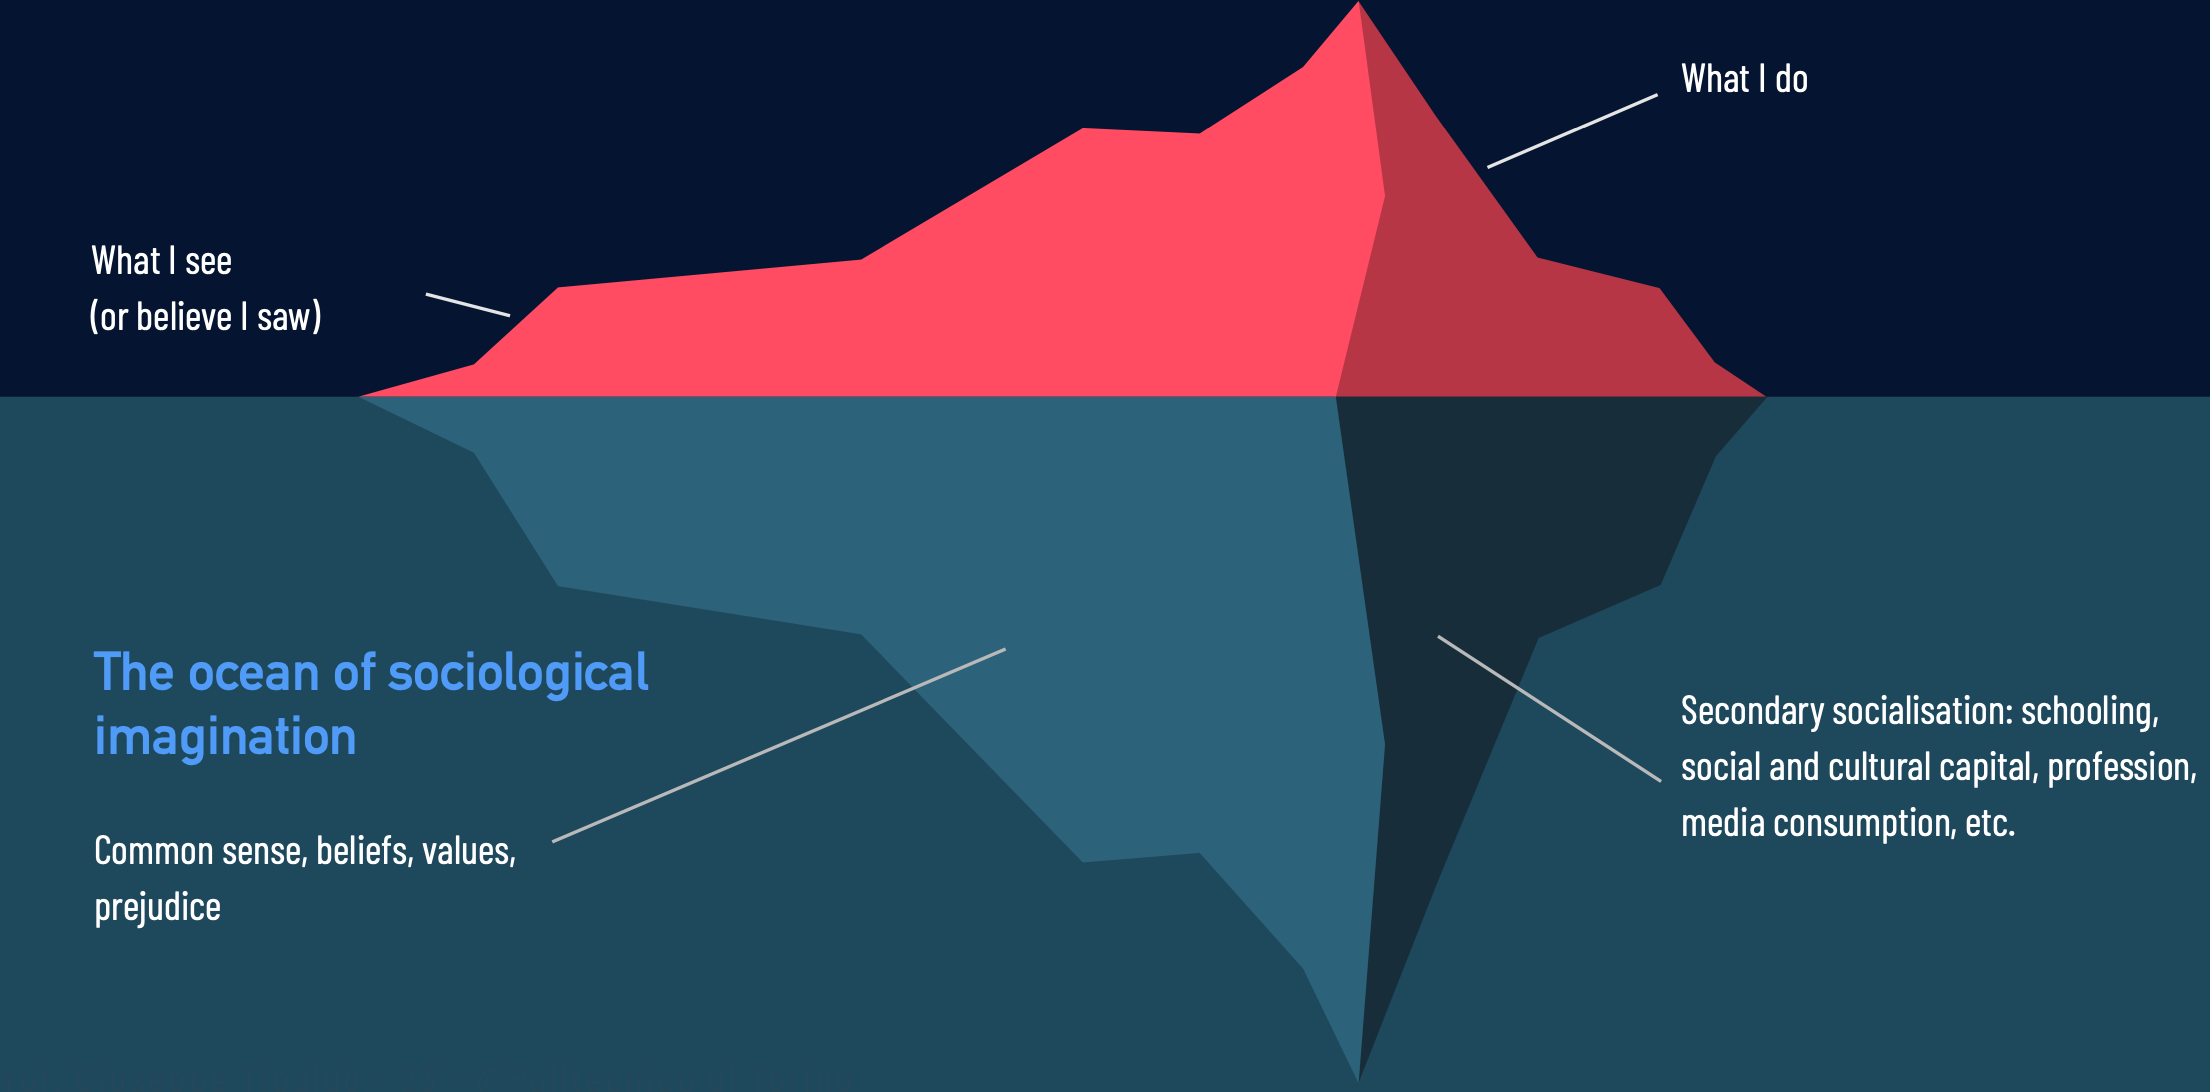
\includegraphics[width=0.5\linewidth]{Images/Sociology/Iceberg.png}
    \caption{The Iceberg Relation}
    \label{fig:Sociology_Iceberg}
\end{figure}

\section{Nomina Nuda Tenemus}
“Nomina Nuda Tenemus” \footnote{This phrase is notably referenced in Umberto Eco’s The Name of the Rose, where it highlights the importance of meaning beyond mere names.} translates to “we hold only bare names.” It suggests that without deeper understanding or context, words are merely empty labels. 
Without a clear name or definition—in this case, within the realm of cybersecurity—it becomes impossible to identify what needs protection. Moreover, this lack of clarity prevents the formulation of an effective legal framework.
\subsection{Overview of Cybersecurity}
The diagram \ref{fig:Overview} provides an overview of cybersecurity from a sociological perspective, broken down into two main sections: Definitions and Terminologies and Concepts. Here's an explanation of each component:
\begin{itemize}
    \item Definitions: This section focuses on defining key concepts like cybercrime and cybersecurity. It includes an analysis of the historical development of these fields and discusses current trends in cyber threats and protection strategies.
    \item Terminologies and Concepts: This section introduces foundational terms necessary for understanding cybersecurity, such as malware, phishing, and ransomware. It highlights the necessity of a shared vocabulary for precisely identifying and describing cyber threats, offering structured classifications and comprehensive definitions of cybercrime.
\end{itemize}

\begin{figure}[H]
    \centering
    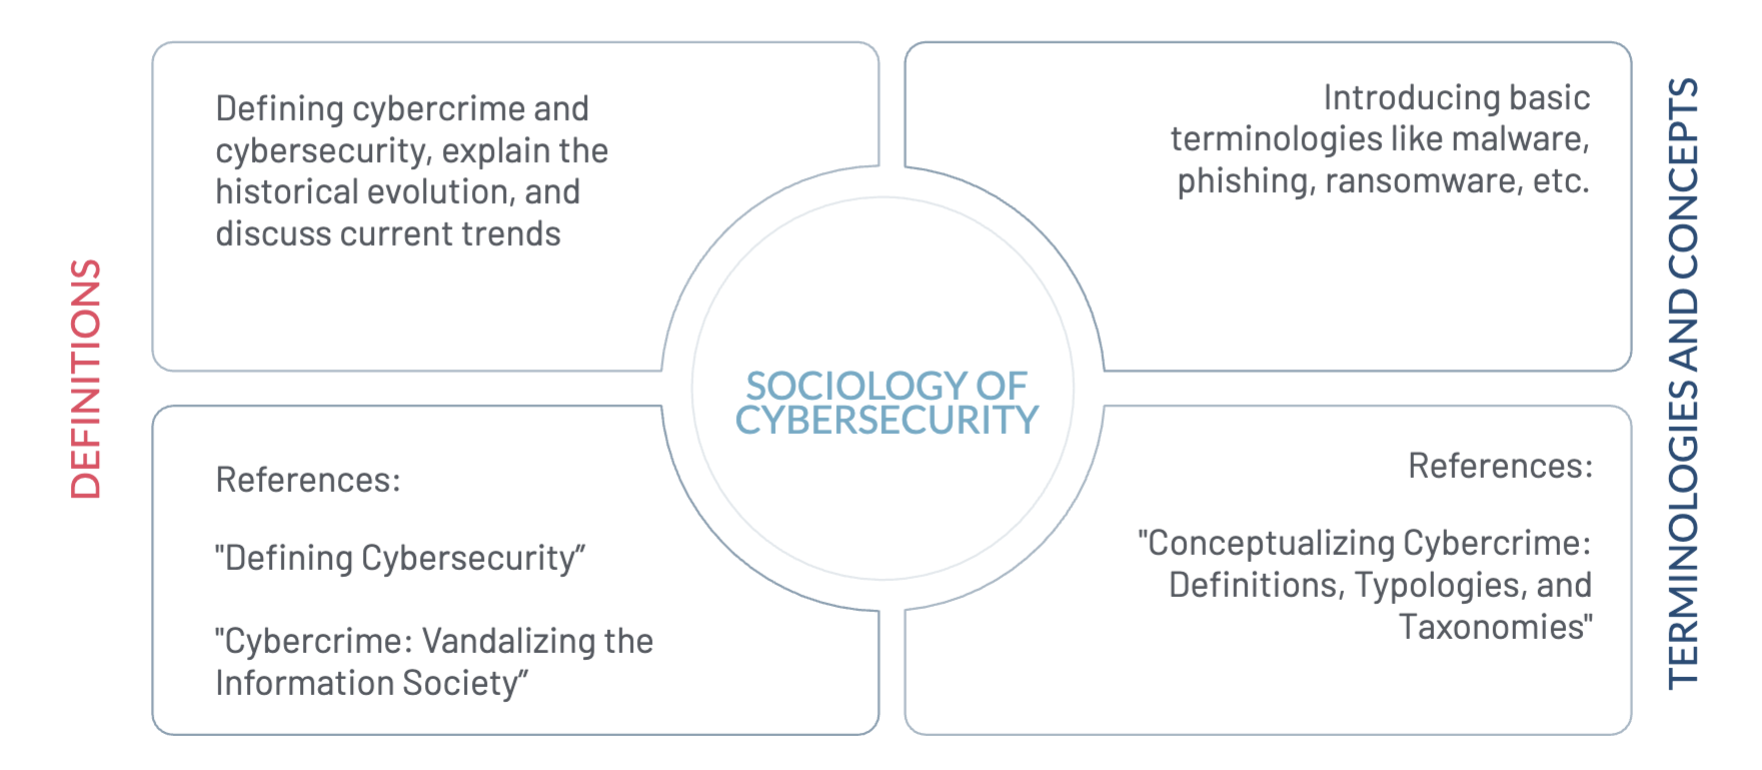
\includegraphics[width=0.5\linewidth]{Images/Sociology/Overview.png}
    \caption{Overview of Cybersecurity from a sociological perspective}
    \label{fig:Overview}
\end{figure}

\subsection{Definitions of Cybercrime}
\subsubsection{Vocabulary}
Figure \ref{fig:Vocabulary1} illustrates how the vocabulary used to describe similar phenomena has changed over time. Nowadays, cybercrime attacks are a top priority on the agenda of many countries.
\begin{figure}[H]
    \centering
    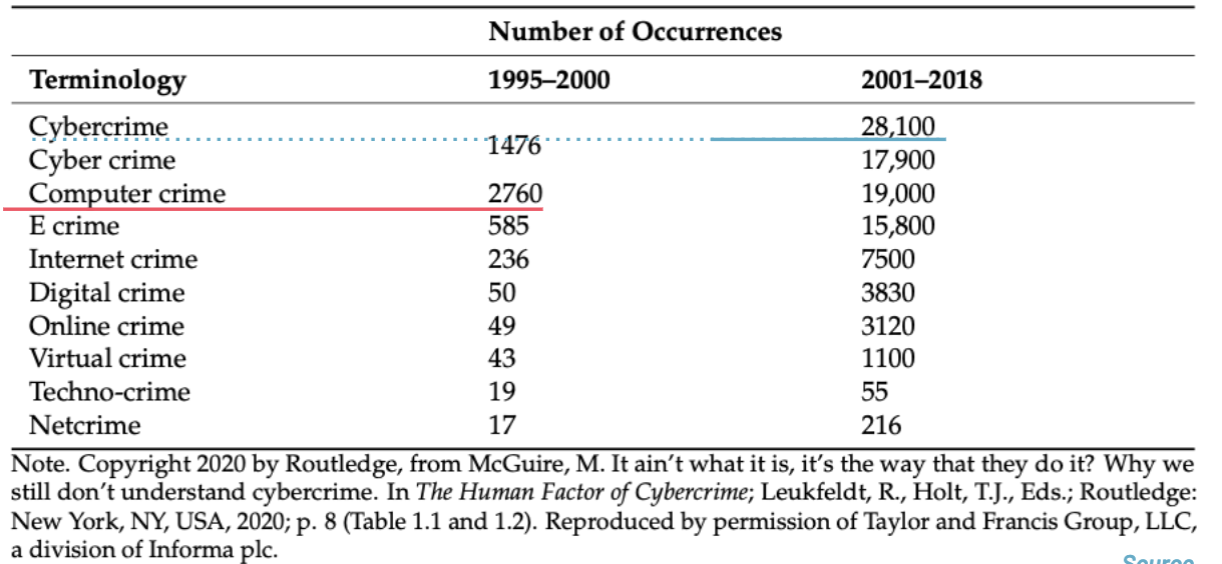
\includegraphics[width=0.5\linewidth]{Images/Sociology/Vocabulary1.png}
    \caption{Cybercrime terminology in the periods 1995-2000 and 2001-2018}
    \label{fig:Vocabulary1}
\end{figure}

\subsubsection{Official Definitions}
Figure \ref{fig:Definitions} illustrates a shift from material to immaterial concerns regarding cybercrime attacks. In 1994, the United Nations issued the first official document, although cybercrimes already existed at that time, even if they were not yet formally named. Initially, cybercrimes were strictly related to the computer sphere. Over time, however, the definition of cybercrime expanded to encompass a broader range of activities, incorporating various new aspects. The main points of the new definitions are: data processed by computer systems or networks and information systems, either as a primary tool or as a primary target.

\begin{figure}[H]
    \centering
    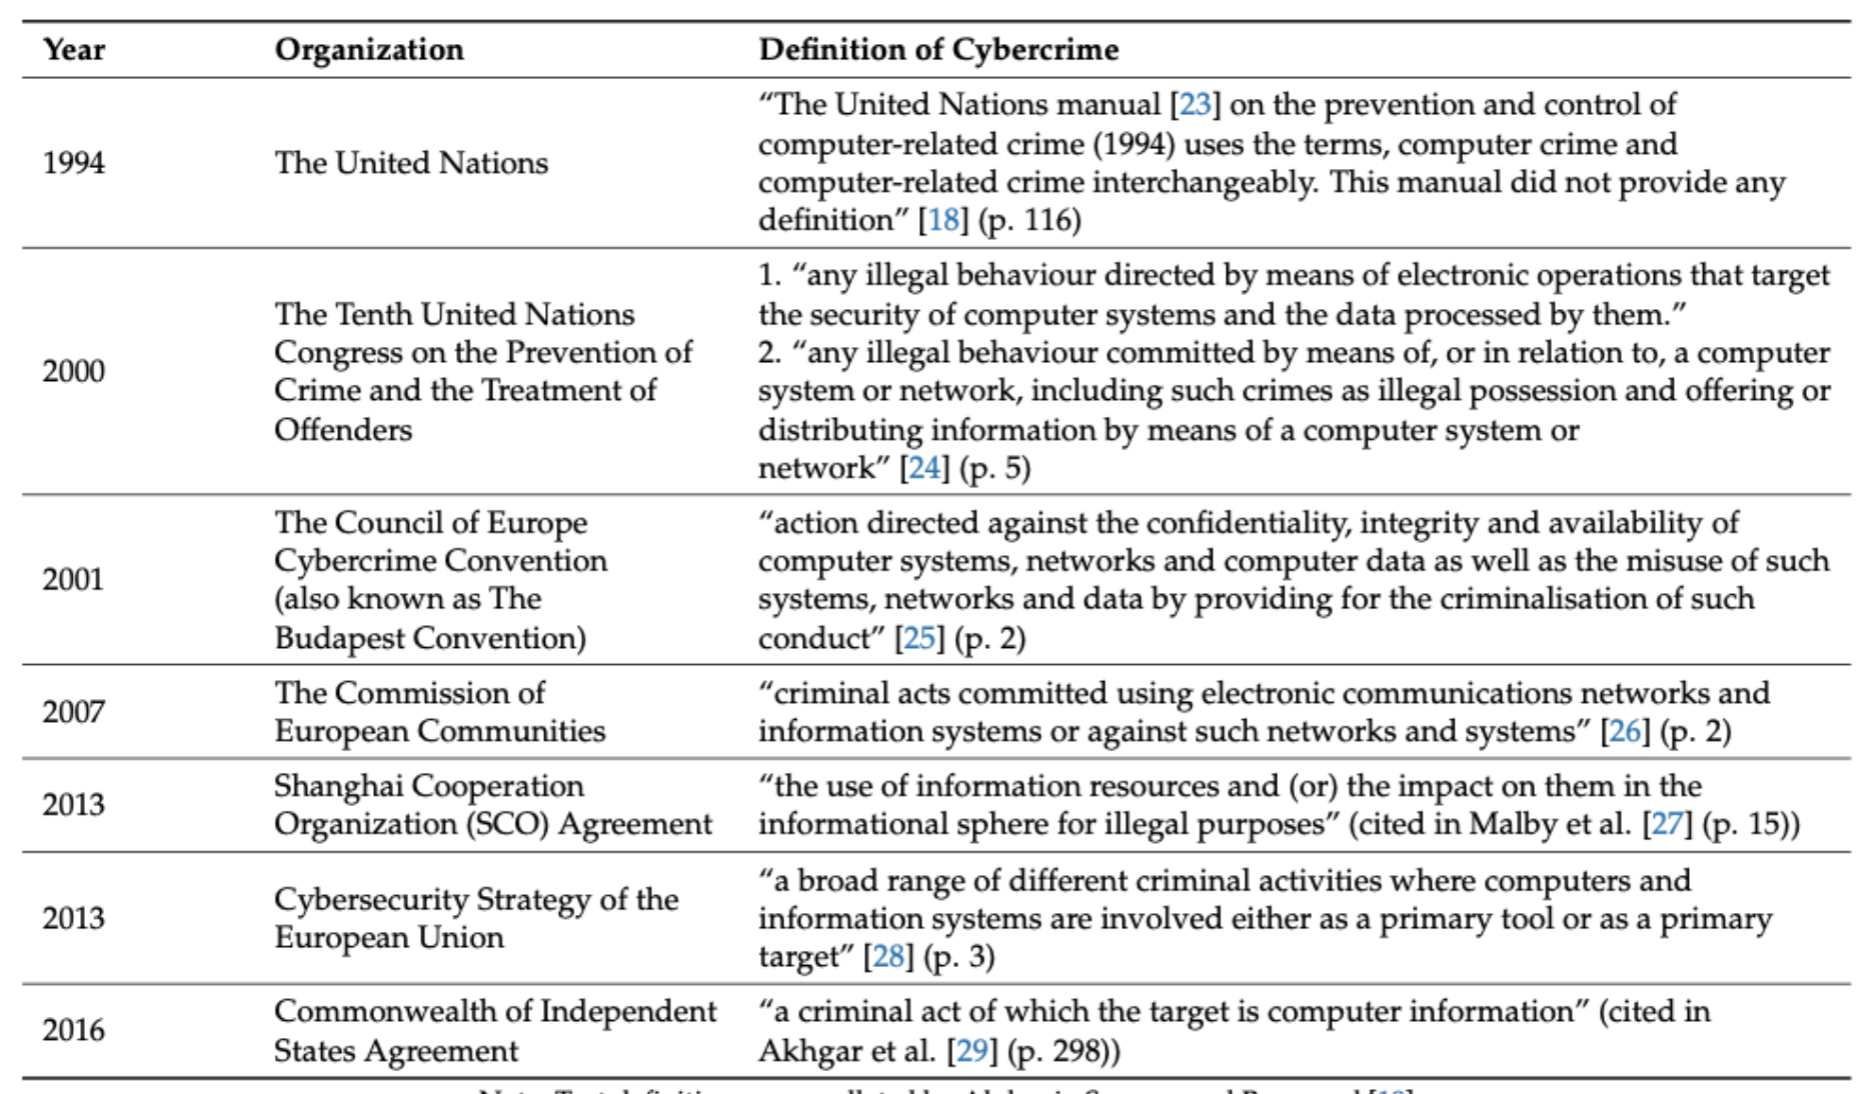
\includegraphics[width=0.5\linewidth]{Images/Sociology/Definitions.png}
    \caption{Organization definitions of cybercrime}
    \label{fig:Definitions}
\end{figure}

\subsubsection{Dichotomous Definitions}
\begin{multicols}{2}
    In research and policymaking, a distinct dichotomy was established. A discrete categorical approach was applied to define cybercrimes, classifying them as either cyber-enabled or cyber-dependent. Cyber-enabled crimes are traditional offenses that predate the advent of technology but are now facilitated or made easier (i.e., enabled) by digital technology. Cyber-dependent crimes are crimes that arose with the advent of technology and cannot exist (i.e., dependent) outside the digital world. 
    \columnbreak

    Many people also agree with another, non-discrete dichotomy from a continuum approach perspective. The continuum approach to cybercrimes views cybercrime not as a discrete category but as a spectrum, where offenses range from traditional crimes that are cyber-enabled to those that are fully cyber-dependent. Crimes of Type 1 are more technical in nature, while crimes of Type 2 involve more human interaction.

\end{multicols}

\begin{multicols}{2}
    \begin{figure}[H]
        
\includegraphics[width=\linewidth]{Images/Sociology/CategoricalApproach.png}
        \caption{Categorical approach to cybercrime}
    \end{figure}
    \columnbreak
    
    \begin{figure}[H]
        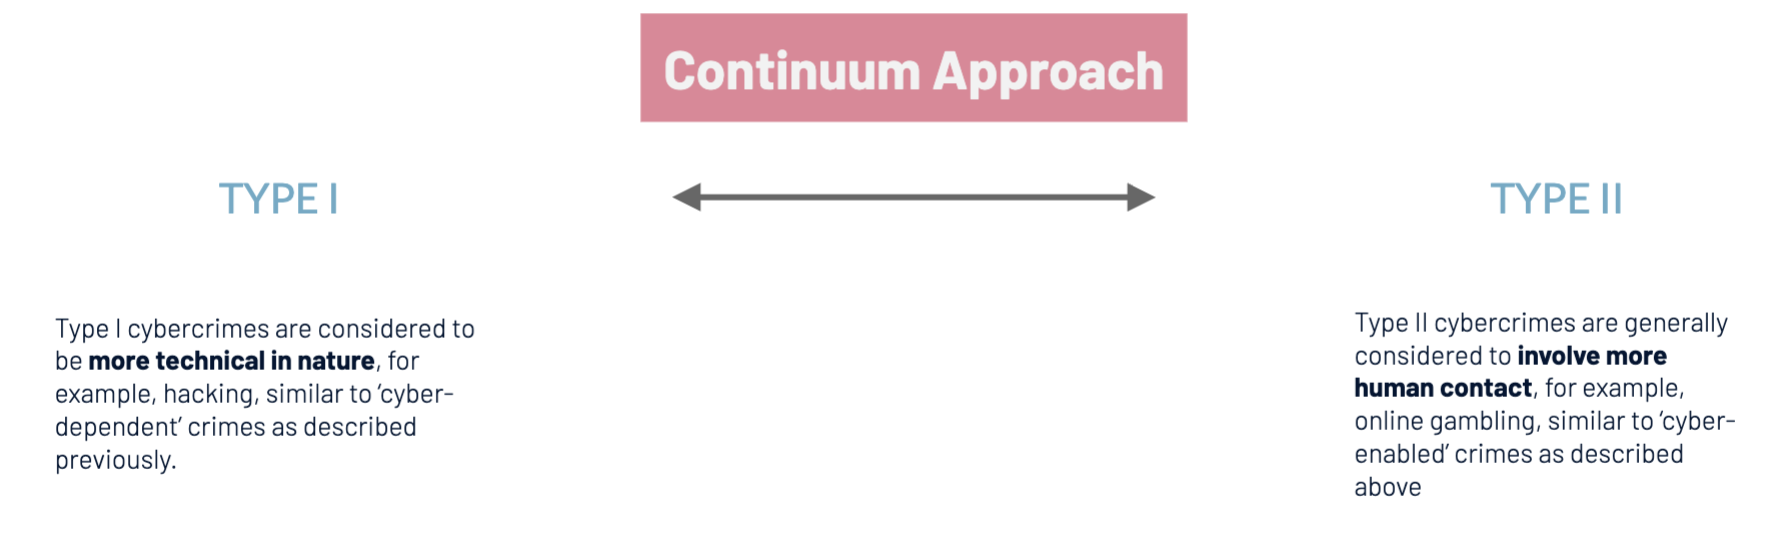
\includegraphics[width=\linewidth]{Images/Sociology/ContinuumApproach.png}
        \caption{Continuum approach to cybercrime}
    \end{figure}

\end{multicols}

\subsubsection{Trichotomous Definitions}
Industries have also attempted to classify clusters of crimes using trichotomous definitions within a categorical approach. First, we analyze the one made by David S. Wall in 2007. Wall introduced three sections:
\begin{itemize}
    \item Crimes against the machine: Computer integrity crimes (e.g., hacking).
    \item Crimes in the machine: known as computer content crimes (e.g., online hate).
    \item Crimes using the machine: Computer-assisted crimes (e.g. piracy).
\end{itemize}
The EU Commission also released labels in 2013 addressing cybercrimes, which share many similarities with the ones presented above. In fact, cybercrimes were divided in three stages: offenses unique to computers and information systems, content-related offenses and traditional offenses.

\subsection{Cybersecurity is}

As stated by Fredrick Chang, former Director of Research at the National Security Agency in the United States:
\begin{quotation}
    A science of cybersecurity offers many opportunities for advances based on a \textbf{multidisciplinary approach}\footnote{Crimes concern many fields of phenomena.}, because, after all, cybersecurity is fundamentally about an \textbf{adversarial engagement}. Humans must defend machines that are attacked by other humans using machines. So, in addition to the critical traditional fields of computer science, electrical engineering, and mathematics, perspectives from other fields are needed.
\end{quotation}

Analyzing literature\footnote{Craigen et al.2014} "Cyber" is a prefix connoting cyberspace and refers to electronic communication networks and virtual reality.
The term "cyberspace" describes a vision of a three-dimensional space of pure information, moving between computer and computer clusters where people are generators and users of the information. Public Safety Canada\footnote{2010} defines cyberspace as:

\begin{quotation}
    The electronic world created by interconnected networks of information technology and the information on those networks. It is a global common where people are linked together to exchange ideas, services, and friendships.
\end{quotation} 

Cyberspace is a dynamic mixed-reality\footnote{The *phygital* reality. A funsion of physical and digital realities} environment where hardware is significant, as it hosts real interactions. 

\vspace{0.5cm}

\noindent In addition, cybersecurity must necessarily include and seek to understand:
\begin{itemize}
    \item Who securitizes, identifying the actors and entities responsible for enforcing security.
    \item What issues, specifying the particular assets, systems, or information at risk.
    \item For Whom, clarifying the stakeholders, such as individuals, organizations, or governments, who benefit from the security measures
    \item Why, analyzing the motivations behind security implementations, whether they are economic, political, or social
    \item with What results, evaluating the effectiveness and outcomes of the security strategies applied
    \item under What conditions (structure), defining the structural or environmental factors influencing the security landscape
    \end{itemize}

\subsection{Cybersecurity Definitions}
\textbf{Defensive perspective}

\begin{enumerate}
    \item Cybersecurity consists largely of defensive methods used to detect and thwart would-be intruders. (Kemmerer, 2003)
    \item Cybersecurity entails the safeguarding of computer networks and the information they contain from penetration and from malicious damage or disruption. (Lewis, 2006)
    \item Cybersecurity is the collection of tools, policies, security safeguards, guidelines, risk management approaches, training, best practices, assurance and technologies that can be used to protect the cyber environment and organization and user's assets. (ITU, 2009)
    \item The ability to protect or defend the use of cyberspace from cyber-attacks. (CNSS, 2010)
    \item The state of being protected against the criminal or unauthorized use of electronic data, or the measures taken to achieve this. (Oxford University Press, 2014)
    \item The activity or process, ability or capability, or state whereby information and communications systems and the information contained therein are protected from and/or defended against damage, unauthorized use or modification, or exploitation. (DHS, 2014)
\end{enumerate}

\textbf{Continuous perspective}\footnote{Ability to survive and adapt over time} and \textbf{Ecosystem perspective}

\begin{enumerate}
    \setcounter{enumi}{7}
    \item The body of technologies, processes, practices and response and mitigation measures designed to protect networks, computers, programs and data from attack, damage or unauthorized access to ensure confidentiality, integrity and availability. (Public Safety Canada, 2014)
\end{enumerate}

\textbf{Risk perspective}

\begin{enumerate}
    \setcounter{enumi}{8}
    \item Cyber Security involves reducing the risk of malicious attack to software, computers and networks. This includes tools used to detect break-ins, stop viruses, block malicious access, enforce authentication, enable encrypted communications, and on and on. (Amoroso, 2006)
\end{enumerate}

\textbf{Sociepistemic definition} \footnote{Examines how knowledge is created, validated, and shared within social contexts.} - the 10th defintion
\begin{enumerate}
    \setcounter{enumi}{9}
    \item Cybersecurity is the organization and collection of \textbf{resources, processes, and structures} used to \textbf{protect} cyberspace and cyberspace-enabled systems from \textbf{occurrences} that \textbf{misalign} de jure from de facto \textbf{property rights}.
\end{enumerate}
\clearpage
The last definition comprehend four key dimensions:
\begin{multicols}{2}
    \centering "the organization and collection of \textbf{resources, processes, and structures}"

    \columnbreak

    \textbf{Complexity}
        \newline Complex interactions among humans, between systems and between humans and systems.

\end{multicols}
    

\begin{multicols}{2}
    \centering "used to \textbf{protect} cyberspace and cyberspace-enabled systems"

    \columnbreak

    \textbf{Extensiveness}
        \newline Protection from all threats, including intentional, accidental, and natural hazards.

\end{multicols}

\begin{multicols}{2}
    \centering "from \textbf{occurrences}"

    \columnbreak

    \textbf{Unpredictability}
        \newline Threats can also be unpredictable, often arising unexpectedly and in forms that are difficult to anticipate or prepare for.

\end{multicols}


\begin{multicols}{2}
    \centering "\textbf{misalign} de jure from de facto \textbf{property rights}"

    \columnbreak

    \textbf{Ownership}
        \newline Any event or activity that causes a misalignment between actual (de facto) property rights and perceived (de jure) property rights, whether intentional or accidental. i.e. "The system does not work properly".

\end{multicols}


\subsection{Terminologies and Concepts}

\raggedright
There is a need to scrutinize the evolving landscape of technology that brings with it new cybercriminal behaviors.

\raggedleft \textit{Society is the domain we aim to study.}

\begin{figure}[H]
    \centering
    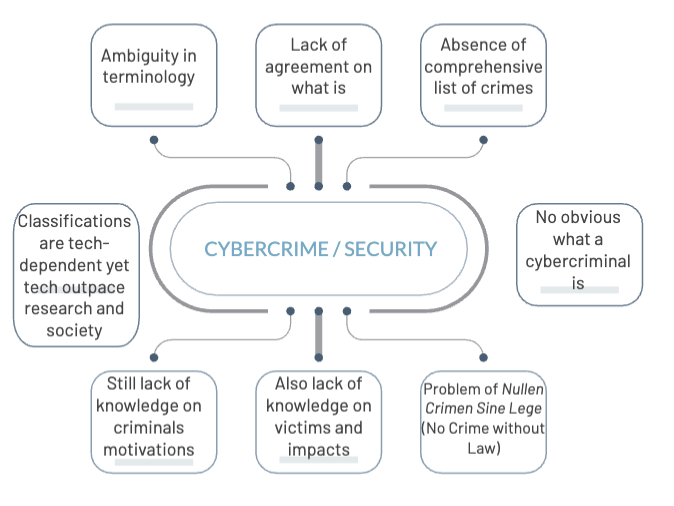
\includegraphics[width=0.5\linewidth]{Images/Sociology/securityLimits.png}
    \caption{Limits and key challenges of cybercrime and cybersecurity}
    \label{fig:cyberLimits}
\end{figure}

\centering
\textit{Be aware: today, the spread of knowledge is also influenced by public opinion and various sociological and political factors.}
\raggedright

\chapter{Social Engineering}

\section*{What is Social Engineering?}

SE has two different meanings according to dictionaries: 
\begin{enumerate}
    \item \textbf{Social and Political Sciences}: the use of centralized planning in an attempt to manage social change and regulate the future development and behavior of a society.
    
    \vspace{0.1cm}

    There is a need for experts to create social or economic policies, as these are not tasks that everyone can undertake.
    \[
        \text{SE as Policy-making strategy.}
    \]
    \item \textbf{Cyberspace}: the use of deception to manipulate individuals into divulging confidential or personal information that may be used for fraudulent purposes.
\end{enumerate}

\subsection*{Common Semantic Dimensions}
\begin{center}
    Hatfield, 2017.
\end{center}
\raggedcolumns
\begin{multicols}{2}
    \begin{center}
    \textbf{Epistemic asymmetry}
    \end{center}
    "Knowledge" asymmetry.

    Occurs when one person or group enjoys a \textit{significant advantage in terms of knowledge} over another person or group \textit{within a specific domain} to which that knowledge applies. 

    \vspace{0.1cm}

    \textcolor{Red}{||} Doesn't necessarily imply a technocratic dominance.\textcolor{Red}{||}

    \vspace{0.2cm}
    For example, what we typically experience with professors.

    \columnbreak

    \begin{center}
    \textbf{Teleological replacement}
    \end{center}
    "Purpose", "end".

    Occurs when person or group A successfully substitutes the original purpose or goal of individual or group B’s behavior with their own.

    \vspace{0.1cm}

    We can say, “My goals become your goals” (implementing a social strategy that contradicts your aims).
    
\end{multicols}

    \begin{center}
        \textbf{Technocratic dominance}
        \end{center}
    
        Occurs when a person or group possessing a high-degree of technical knowledge uses that knowledge to \textit{enact changes in the behavior of others}, where such behaviors place \textit{those affected in a position of decreased power or authority} relative to the former within the affected domain.
        
        \vspace{0.1cm}
    
        One consequence of this in the STS\footnote{Multidisciplinary field that studies the conditions under which science and technology develop, and how these developments shape society, politics, and culture.} domain is the \textit{Knowledge Deficit} Model: The more ignorant you are, the more you fear and refuse to accept advancements.
            
        \vspace{0.1cm}
    
        A side effect of an originally very good solution (which clashes with the ideas of liberal democracy), referencing the San Mathews effect\footnote{In the context of social sciences, the term is sometimes used to describe the negative consequences of rapid, unplanned urban development, such as increased social stratification, lack of infrastructure, or economic disparity.}.

        \vspace{0.1cm}
    
        \textcolor{Red}{||} It is a choice, based on your knowledge.\textcolor{Red}{||}
    
\section{The Definition}
Political social engineering and technological social engineering are different phenotypical expressions of the same underlying genotype, characterized by epistemic asymmetry, technocratic dominance, and teleological replacement.

As technical security measures increased in their sophistication, "computer hackers", began to rely more and more on non-technical methods to achieve their goals. 

\subsection*{Key features of social engineering attacks}
\begin{enumerate}
    \item Psychological manipulation.
    \item Tech illiteracy and lack of critical sense (Naivety or curiosity).
    \item Exploitation of trust.
    \item Use of fear or urgency: self/business-protection. 
    \item Impersonation.
    \item Propaganda and misinformation.
    \[
        \textit{"The scandal becomes the message itself."}
    \]
    \item Organizational/Cultural level: exploitation of group dynamics (Sometimes, the dynamics of power hierarchies suppress people’s instinct to protect others).
    \item Media arena: exploitation of the media to spread false information (Also decontextualizing).
    \[
        \textit{"How nothing becomes everything."}
    \]
    \item Procedural failures: lack of security protocols or poor implementation.
\end{enumerate}

\subsection*{Preventing Social Engineering Attacks}

To prevent social engineering attacks, individuals and organizations can:
\begin{itemize}
    \item Educate employees about the risks and signs of social engineering.
    \[
        \textit{The Human is the weakest part of a modern system.}
    \]
    \item Implement strict verification processes for sensitive information requests.
    \item Use multi-factor authentication to add an extra layer of security.
    \item Regularly update and patch systems to protect against vulnerabilities.
    \item Encourage a culture of skepticism and caution regarding unsolicited communications.
\end{itemize}

\vspace{0.5cm}

\begin{center}
    \textit{"The greatest asset of a hacker is not their computer, but their ability to manipulate people."}
\end{center}

\vspace{1 cm}

\begin{center}
    \textbf{A technician or security professional must indeed study aspects of human behavior and psychology.}
\end{center}

\section{Cialdini's Principles}
The book \textit{"Influence: Science and Practice"} (by Robert Cialdini, 1984) outlines six principles of persuasion that can be used to influence people's behavior. These principles are:
\begin{enumerate}
    \item \textbf{Reciprocity}: People feel obligated to return a favor (it's not a simple exchange of resources, but a social norm).
    
    \hspace{1cm} \textit{Example: An attacker might offer a gift to a target, making the target feel obligated to reciprocate by providing personal information.}
    \item \textbf{Commitment and Consistency}\footnote{Consistency is not intended to be morally adequate or coherent, but rather as a proxy for believing and trusting someone else. Consistency is treated as a strategy, requiring effort to maintain or escape from. }: Once people commit to something, they tend to follow through to remain consistent with their commitment. When someone’s mindset or behavior is not aligned with their actions or beliefs (cognitive dissonance), they will often change their beliefs to match their actions. Protecting behaviors by ignoring inconsistencies (neglecting the truth) is a common defense mechanism to maintain psychological stability.

    \hspace{1cm} \textit{Example: Attackers might use a small request (foot-in-the-door technique) to make a target agree to larger requests later. The initial small agreement sets a commitment, which makes further compliance more likely.}

    \item \textbf{Social Proof}: People look to others to determine how to behave, especially in ambiguous situations.
    
    \hspace{1cm} \textit{Example: Attackers might use fake testimonials or reviews to make the scenario as credible as possible, convincing the target that others have benefited from their scam.}
    
    \item \textbf{Authority}: People tend to obey authority figures, even if they are asked to perform objectionable acts.
    
    \hspace{1cm} \textit{Example: Attackers might impersonate a figure of authority, such as a police officer or IT technician, to gain the target's trust and compliance.}

    \item \textbf{Liking} ("influencers principle" in the digital age): People are more likely to be influenced by people they like.
    
    \hspace{1cm} \textit{Example: Attackers might build rapport with the target by finding common interests or using flattery to make the target more receptive to their requests.}

    \item \textbf{Scarcity}\footnote{Not just a material scarcity, but also a psychological one (e.g. toxic relationships).}: People are more likely to desire something if they believe it is scarce or in limited supply.
    
    \hspace{1cm} \textit{Example: Attackers might create a sense of urgency by claiming that an offer is available for a limited time (scarcity) or that a product is in high demand, prompting the target to act quickly.}

\end{enumerate}

\section{SE - Old and New Techniques}
\begin{center}
    In order to configure a taxonomy of social engineering attacks.
\end{center}
\begin{itemize}
    \item Impersonation ("faking an identity"): pretending to be someone else to gain access to sensitive information.
    \item 3RD Party Authorization: occurs when authentication details are stolen by or given to a third party.
    \item Phishing: sending fraudulent emails or messages to trick people into revealing personal information.
    \item POP-UPS: fake alerts or notifications (grab immediate attention) that trick users into clicking on malicious links.
    \item Dumpster Diving: Searching through trash to find sensitive information. An upgrade could involve searching through social media.
    \item Improper Use of Social Media: Sharing sensitive content (often poorly protected) on social media platforms.
    \item Shoulder Surfing: observing someone over their shoulder. This method exploits the physical proximity to the target to gather sensitive data without the need for technology.
    \item In Person Attack: on-site impersonation or simply utilizing someone's terminal.
    \item Internal SE ("rebalancing the epistemic asymmetry"): occurs when system administrators use social engineering techniques against their own organization.
    \item Reverse Social Engineering: occurs when the attacker convinces the victim to initiate contact.
    \item Automated Social Engineering: uses automated tools (e.g. botnets) to perform social engineering attacks.
    \item Semantic Attacks: unlike direct technical attacks, semantic attacks focus on exploiting misunderstandings or misinterpretations of language, such as word choice, phrasing, or context to manipulate the target.
\end{itemize}

\section{Developing a Framework for Social Engineering Attacks}
\subsection{SE - Kevin Mitnick's Attack Cycle}
\begin{center}
    Kevin Mitnick's Social Engineering Attack Cycle, prototype of a social engineering attack.
\end{center}
The typical cycle involves four stages:
\begin{enumerate}
    \item \textbf{Research}: gathering information about the target, such as personal details, interests, and relationships.
    \item \textbf{Developing Rapport and Trust} (the social part): building a relationship with the target to gain their trust and cooperation.
    \item \textbf{Exploiting Trust}: using the established rapport to manipulate the target into divulging sensitive information or performing actions that benefit the attacker.
    \item \textbf{Utilize Information}: using the information obtained to further exploit the target or carry out additional attacks.
\end{enumerate}


\begin{figure}[H]
    \centering
    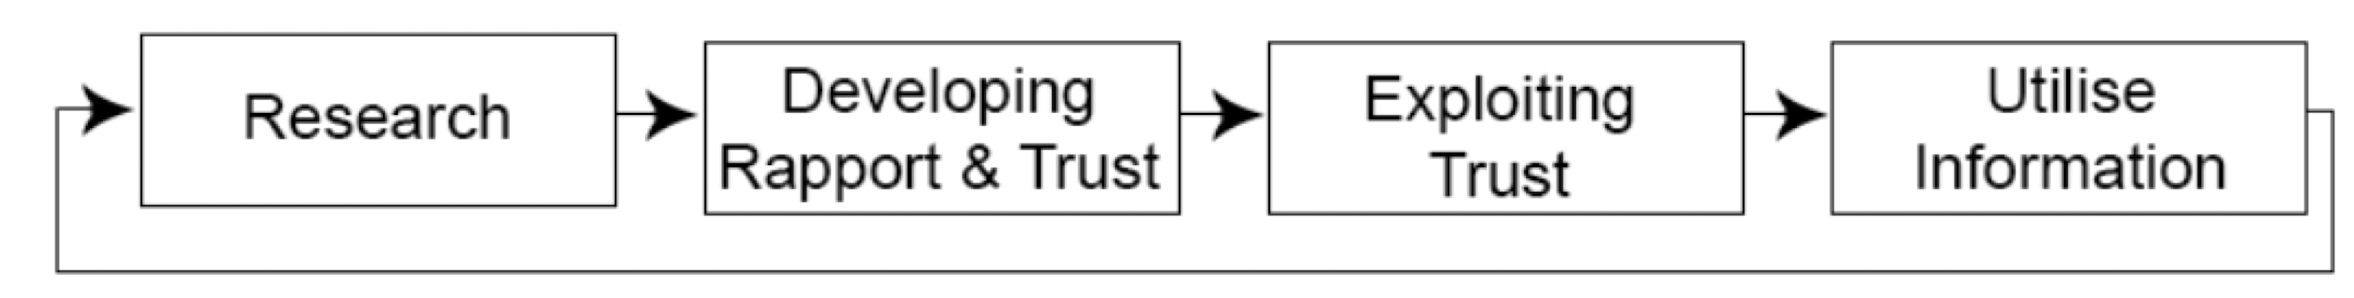
\includegraphics[width=0.7\linewidth]{Images/Sociology/SEcycle.png}
    \caption{Kevin Mitnick's Social Engineering Attack Cycle}
\end{figure}

\subsection{SE - Ontological Model}
The diagram \ref{fig:SEonto} outlines the components and relationships involved in a social engineering attack. The core of the schema is the attack itself, referred to as “the event.”

This central event connects key elements, including the social engineer (the attacker), the target (the victim), the medium (the communication channel), the techniques employed, the compliance principles exploited, and the goal of the attack. Each component plays a distinct role in the orchestration and execution of the attack.

\begin{figure}[H]
    \centering
    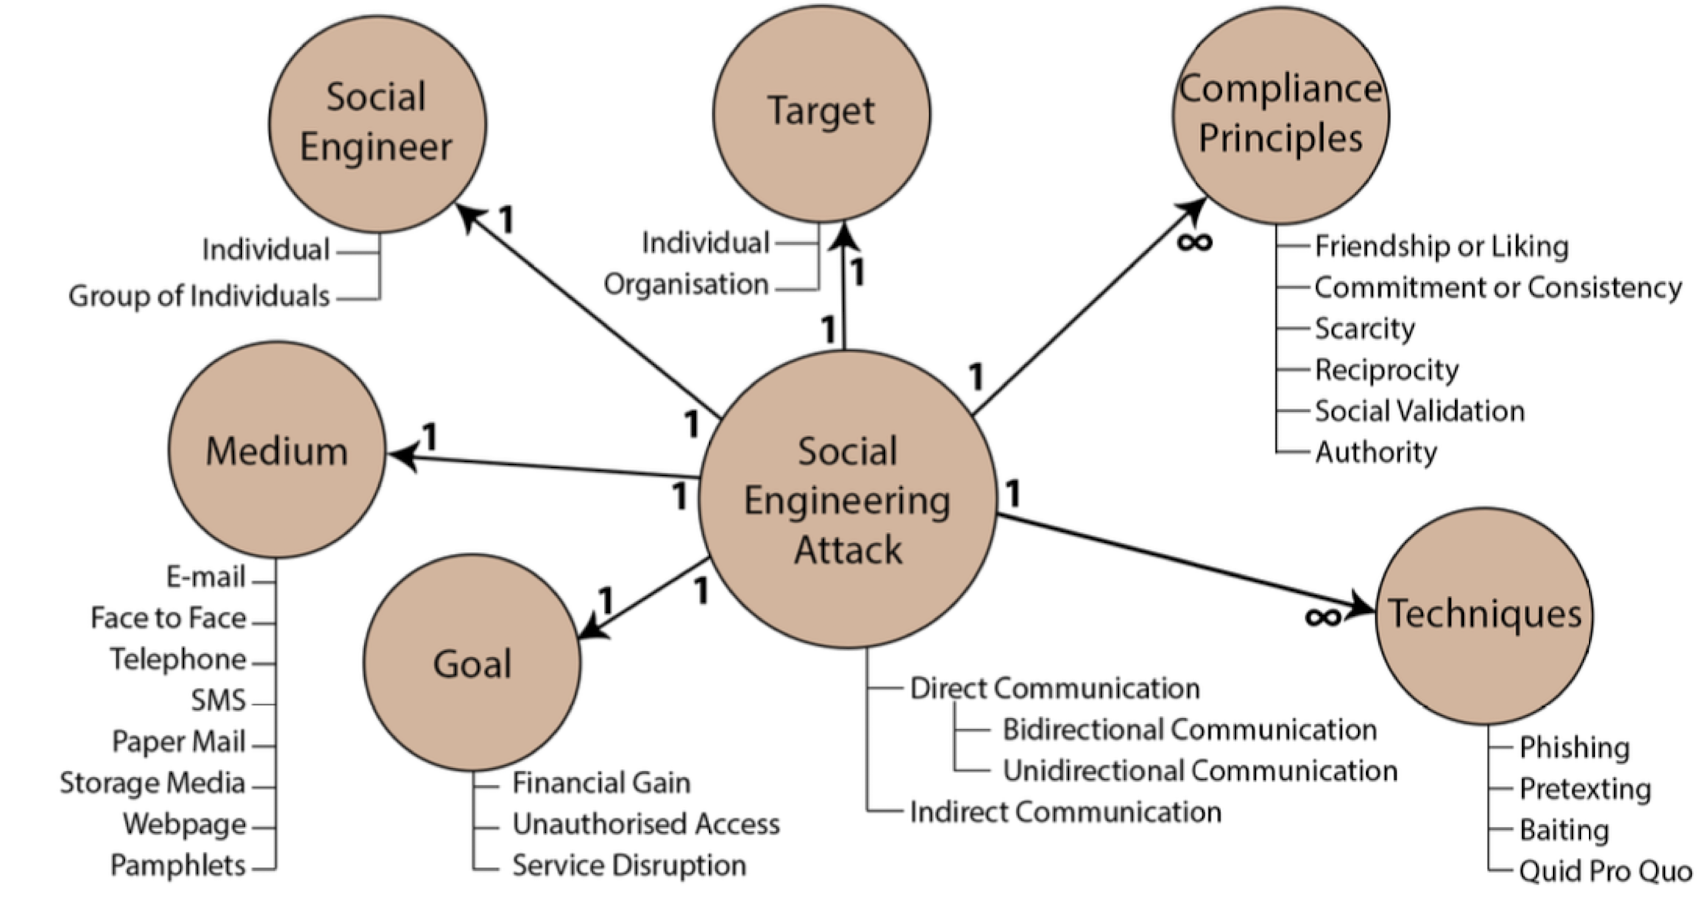
\includegraphics[width=0.7\linewidth]{Images/Sociology/SEonto.png}
    \caption{Ontological Model of Social Engineering}
    \label{fig:SEonto}
\end{figure}

\subsection{SE - Attack Framework}
The figure \ref{fig:SEframework} illustrates a comprehensive framework for social engineering attacks, which includes the following components:
\begin{itemize}
    \item \textbf{Preparation}: analyzing and synthesizing gathered information.
    \begin{itemize}
        \item Combination and analysis of gathered information.
        \item Development of an attack vector: The attacker formulates a specific strategy or approach to exploit the target effectively.
    \end{itemize}
\end{itemize}

\begin{multicols}{2}
    \begin{itemize}
        \item \textbf{Information Gathering}:
        \begin{itemize}
            \item Identify potential sources.
            \item Gather information from sources.
            \item Assess gathered information: Evaluating the quality, relevance, and utility of the collected data.
        \end{itemize}
        \item \textbf{Attack Formulation}: This stage transitions from data collection to defining the objectives and scope of the attack.
        \begin{itemize}
            \item Goal identification.
            \item Target identification.
        \end{itemize}
        
    \end{itemize}

    \columnbreak

    \begin{figure}[H]
        \centering
        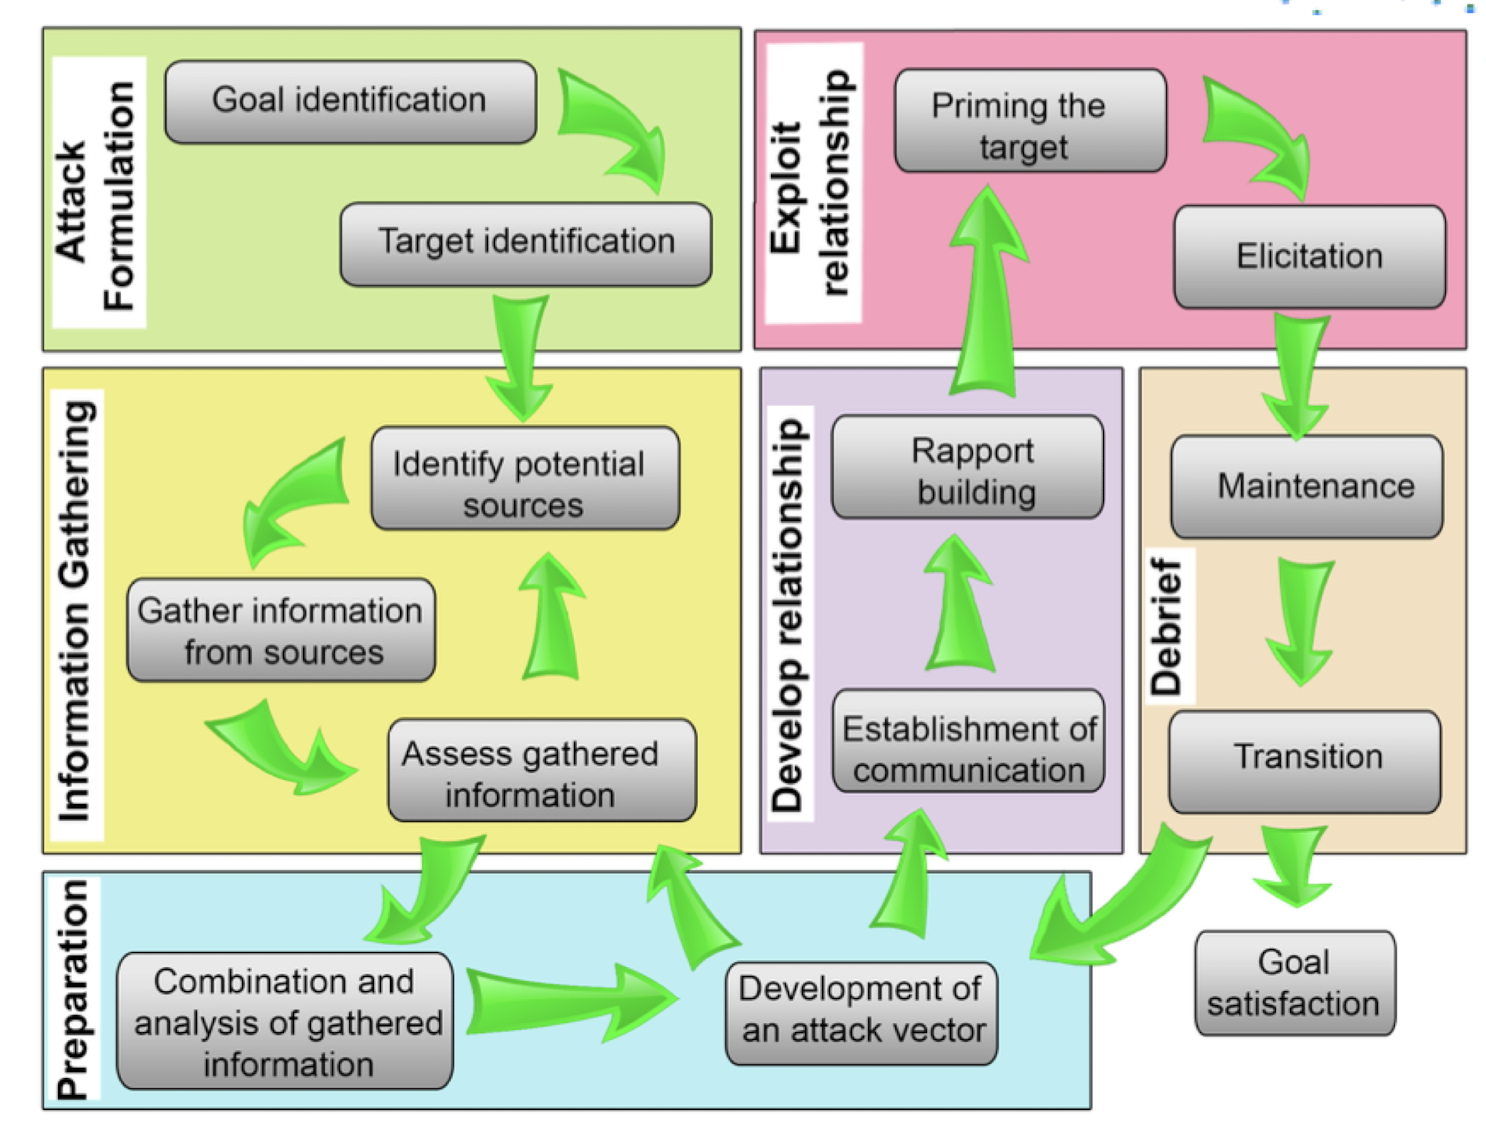
\includegraphics[width=\linewidth]{Images/Sociology/SEframework.png}
        \caption{Social Engineering Attack Framework}
        \label{fig:SEframework}
    \end{figure}
    
\end{multicols}


\begin{itemize}
    \item \textbf{Develop Relationship}: Establishing trust and rapport with the target to facilitate manipulation.
        \begin{itemize}
            \item Establishment of communication.
            \item Rapport building.
        \end{itemize}
    \item \textbf{Exploit Relationship}:
    \begin{itemize}
        \item Priming the target: Preparing the target to act in a way that benefits the attacker, often using psychological principles.
        \item Elicitation: Drawing out sensitive or useful information from the target without their awareness.
    \end{itemize}
    \item \textbf{Debrief}: Ensures that the attacker successfully transitions out of the operation and confirms that their goal has been achieved.
    \begin{itemize}
        \item Maintenance: Keeping the relationship or access open for potential future attacks.
        \item Transition: Shifting focus once the primary objective is achieved.
    \end{itemize}
\end{itemize}

\section{More than Tech}
\begin{center}
    Considering critical infrastructures as sociotechnical systems.
\end{center}
\subsection{Sociotechnical Studies}
Interdisciplinary field that explores the interactions between people (social systems) and technology (technical systems). This approach recognizes that technology and society are interdependent and that changes in one system can have significant impacts on the other.

\vspace{0.5cm}

\begin{center}
    \textit{Sociotechnical studies aim to provide a comprehensive understanding of how technology and society coevolve and to inform the design and implementation of technologies that are socially responsible and beneficial.}
\end{center}

\subsubsection*{Cybersecurity and S-T Systems - A Brief History}
The advent of personal computing and the internet in the late 20th century introduced the first major cybersecurity concerns. Initially, efforts were focused \textbf{primarily on technical solutions}, such as firewalls and antivirus software, to combat cyber threats. However, as technology became increasingly embedded in all aspects of society, the scope of cybersecurity expanded to encompass social, cultural, and organizational dimensions.

\vspace{0.5cm}

From early on, the sociotechnical systems (S-T) perspective emphasized that cybersecurity challenges \textbf{cannot be resolved through technical measures alone}. Social factors—such as user behavior, organizational practices, and policy frameworks—play an equally critical role in ensuring robust cybersecurity defenses.

\vspace{0.5cm}

The 2000s saw a dramatic increase in cybercrime. This period underscored the need for a more integrated approach to cybersecurity that incorporates both social and technical dimensions. Research began to focus on issues like user education, insider threats and the socio-economic drivers of cybercrime.

The S-T systems approach became more prominent in cybersecurity research, emphasizing the need to \textbf{design systems that are resilient to both technical exploits and social engineering attacks}.

\vspace{0.5cm}

The current era is characterized by rapid digital transformation, with technologies such as AI, IoT, and big data. As organizations undergo digital transformation, cybersecurity challenges have become more complex and persuasive. There is an increasing focus on the \textbf{ethical implications} of cybersecurity practices, data privacy and the balance between security and civil liberties.

\subsection{Emergent Properties}
Behavior of  sociotechnical system cannot be fully understood by analyzing its components in isolation; \textbf{interactions} between components generate \textbf{new properties}.

In ICT (Information and Communication Technology) systems, the interaction between users, technologies and organizational processes can \textbf{lead to unexpected outcomes}. 